\section{Theorie}
\label{sec:Theorie}
\subsection{Ziel}
Ziel des Versuchs ist die Untersuchung der Fundamentalfrequenzen und Schwebung von gekoppelten Schwingkreisen.
\subsection{Gekoppelte Systeme}
Ein gekoppeltes System beinhaltet zwei Systeme die so miteinander verbunden sind,
dass sie auf einander einwirken und durch die Kopplung Energie austauschen können.
Die Energie von System 1 nimmt ab und gleichzeitig steigt die Energie von System 2.
Das Bestimmen von Frequenz und Amplitude in einem Schwingkreis fällt leichter,
deshalb wird einer in dem Versuch verwendet und nicht bekannte Systeme wie gekoppelte Pendel.\\
\subsection{kapazitiv gekoppelte Schwingkreise}
Wie in Abbildung 1 zu sehen, werden zwei identische Schwingkreise die durch einen Koppelkondensator, also der Kapazität $C_k$,
betrachtet.
  \begin{figure}
    \centering
    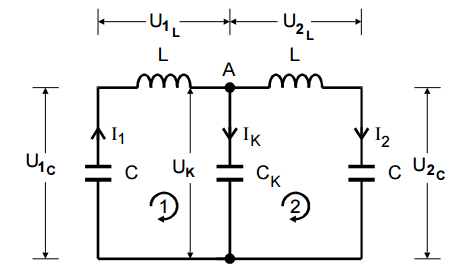
\includegraphics[width=0.7\textwidth]{Prinzipschaltbild.PNG}
    \caption{Schaltbild von zwei kapazitiv gekoppelten Schwingkreisen.\cite{skript}}
    \label{abb:SchaltbildSchwingkreis}
    \end{figure}\\
\newpage
Am Knotenpunkt A gilt laut Kirchhoffscher Knotenregel:\\
 \begin{equation}
   I_k = I_1 - I_2
 \end{equation}\\
 Für die Maschen 1 und 2 gilt:
 \begin{align}
  0&= U_{1_C} + U_{1_L} + U_K \label{eqn:maschenregel1}\\
  0&= U_{2_C} + U_{2_L} + U_K \label{eqn:maschenregel2}.
 \end{align}\\
 %\eqref{eqn:1} blaaaaablaaa
 %\eqref{eqn:2}hukjhsjkfdnbjrs
Mit $U_L=L\dot{I}$ und $U_C = \frac{1}{C}\int I\, \symup{d}t$ erhält man, nach Einsetzten und Differenzieren nach t, zwei Differentialgleichungen:\\
\begin{align}
  L\ddot{I_1} + \frac{1}{C}I_1 + \frac{1}{C}  (I_1-I_2) =&0\\
  L\ddot{I_2} + \frac{1}{C}I_2 + \frac{1}{C}  (I_1-I_2) =&0.
\end{align}\\
Um die Dgln lösen zu können, werden sie zunächst entkoppelt, dies geschieht durch Addition bzw. Subtraktion der Gleichungen voneinander,
ebenfalls werden die Summe bzw. die Differenz der Ströme als neue Variablen eingeführt:\\
\begin{align}
 L\frac{d^2}{dt^2}(I_1+I_2) + \frac{1}{C}(I_1+I_2)=&0\\
 L\frac{d^2}{dt^2}(I_1-I_2) + \left(\frac{1}{C} + \frac{2}{C_K} \right)(I_1-I_2)=&0.
\end{align}
 Die Lösungen der Gleichungen lauten:\\
 \begin{align}
   (I_1+I_2)(t)&=(I_{1_0}+I_{2_0})\cos\left(\frac{t}{\sqrt{LC}}\right) \label{eqn:loesungen+}\\
   (I_1-I_2)(t)&=(I_{1_0}-I_{2_0})\cos\left(\frac{t}{\sqrt{L\left(\frac{1}{C}+\frac{2}{C_K}\right)^{-1}}}\right) \label{eqn:loesungen-}.
 \end{align}
 Die Schwingungsfrequenzen sind hierbei:
 \begin{align}
   \nu^{+}&=\frac{1}{2\pi\sqrt{LC}} \label{eqn:Frequenz1}\\
   \nu^{-}&=\frac{1}{2\pi\sqrt{L\left(\frac{1}{C}+\frac{2}{C_K}\right)^{-1}}}\label{eqn:Frequenz2}.
 \end{align}
Durch Addition und Subtraktion von \eqref{eqn:loesungen+} und \eqref{eqn:loesungen-}  erhält man für die ursprünglichen Ströme $I_1$ und $I_2$:\\
 \begin{align}
   I_1(t)&=\frac{1}{2}(I_{1_0}+I_{2_0})\cos(2\pi\nu^{+}t)+\frac{1}{2}(I_{1_0}-I_{2_0})\cos(2\pi\nu^{-}t)\label{eqn:strom1}\\
   I_2(t)&=\frac{1}{2}(I_{1_0}+I_{2_0})\cos(2\pi\nu^{+}t)-\frac{1}{2}(I_{1_0}-I_{2_0})\cos(2\pi\nu^{-}t)\label{eqn:strom2}.
 \end{align}
 In dem System von gekoppelten Oszillatoren gibt es zwei Spezialfälle.
 Im ersten Fall werden beide Schwingkreise mit gleicher Amplitude und in Phase ausgelenkt, so gilt $I_{1_0}=I_{2_0}$.
 Die beiden Schwingkreise schwingen dann mit $\nu^{+} $.
 Da sich die Ströme $I_1$ und $I_2$ ständig kompensieren, liegt am Koppelkondensator zu keiner Zeit eine Spannung an.
 Im zweiten Fall sind beide Schwingkreise mit der gleichen Amplitude aber entgegengesetzter Phase ausgelenkt, somit folgt $I_{1_0}=-I_{2_0}$.
 Die beiden Schwingkreise schwingen gegenphasig mit $\nu^{-}$ und am Koppelkondensator liegt eine maximale Spannung an.
 Diese beiden Fälle werden als Fundamentalschwingungen bezeichnet.\\
 \\
 Im Gegensatz dazu stehen die Schwebungen, diese ergeben sich durch auslenken von nur einem Schwingkreis.
 Es gilt zum Beispiel $(I_{1_0}\neq I_{2_0}=0)$ für eine Auslenkung des ersten Schwingkreises.
 Durch Umformungen von den Gleichungen \eqref{eqn:strom1} und \eqref{eqn:strom2} ergeben sich anschließend folgende Gleichungen:
 \begin{align}
   I_1(t)&=I_{1_0}\cos\left(\frac{1}{2}2\pi(\nu^{+}+\nu^{-})t\right)\cos\left(\frac{1}{2}2\pi(\nu^{+}-\nu^{-})t\right)\\
   I_2(t)&=I_{2_0}\sin\left(\frac{1}{2}2\pi(\nu^{+}+\nu^{-})t\right)\sin\left(\frac{1}{2}2\pi(\nu^{+}-\nu^{-})t\right).
  \end{align}
\newpage
Die folgende Abbildung zeigt den Verlauf der Ströme, das System schwingt mit der Frequenz $\frac{1}{2}(\nu^{+}+\nu^{-})\approx\nu^{+}$
und die Amplitude verändert sich mit der Schwebungsfrequenz $\nu^{-}-\nu^{+}$ zwischen den Extremwerten 0 und $I_{1_0}$. Für das Verhältnis gilt:\\
  \begin{equation}
    n=\frac{\nu^+ + \nu^-}{2(\nu^{-} - \nu^{+})}\label{eqn:verhaeltnis}.
  \end{equation}
  \begin{figure}[!h]
    \centering
    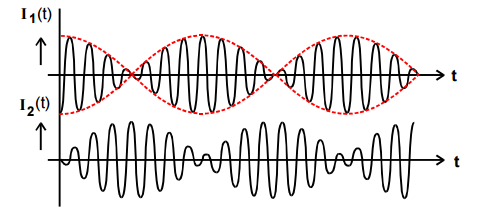
\includegraphics[width=0.7\textwidth]{schwebung.PNG}
    \caption{Verlauf der Ströme im Fall der Schwebung\cite{skript}.}
    \label{abb:schwebung}
    \end{figure}
\\
  Ist die Amplitude von Oszillator 1 maximal und von Oszillator 2 null, so steckt die gesammte Energie im Oszillator 1.
  Mit der Zeit geht diese Energie in Oszillator 2 über, die Verhältnisse kehren sich um. Die Energie schwingt zwischen den beiden Oszillatoren mit der Schwebungsfrequenz hin und her.\\
  \subsection{Strom in Abhängigkeit von der Frequenz}
  Werden zwei gekoppelte Schwingkreise durch eine Sinusspannung zum Schwingen angeregt, so ergeben sich nach Abbildung \ref{abb:schaltbildsinus} und mit Hilfe der Kirchhoffschen Maschenregel die folgende Gleichungen:
  \begin{figure}
    \centering
    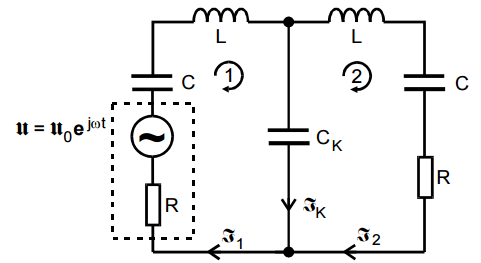
\includegraphics[width=0.6\textwidth]{SchaltbildSinus.PNG}
    \caption{Gekoppelte Schwingkreise mit Sinusgenerator\cite{skript}}
    \label{abb:schaltbildsinus}
    \end{figure}\\
  \begin{align}
    \text{Kreis 1:}\ \ \ U&=(Z_C+Z_L+Z_{C_R}+Z_R)I_1-Z_{C_K}I_2\\
    \text{Kreis 2:}\ \ \ 0&=(Z_C+Z_L+Z_{C_R}+Z_R)I_2-Z_{C_K}I_1.
  \end{align}
Für die Impedanzen gilt:\\
\begin{center}$Z_C=-j\frac{1}{\omega C}$,\ \ \ $Z_L=j\omega L $,\ \ \ $Z_{C_K}=-j\frac{1}{\omega C_K}$,\ \ \ $ZC=R$.
\end{center}
Nach Elimination von $I_1$ und weiteren Rechnungen wie die Trennung in Real- und Imaginärteil, ergibt sich folgendes für den Betrag von $I_2$:\\
\begin{equation}
  \lvert I_2 \rvert = \lvert U \rvert \frac{1}{\sqrt{4\omega^{2}C_K^{2}R^{2}Z(\omega)^{2}+\left(\frac{1}{\omega C_K}-\omega C_KZ(\omega)^{2}+\omega R^{2}C_K\right)^{2}}}.
\end{equation}\\
Anhand dieser Gleichung lässt sich erkennen, dass $I_2$ für $\omega$ \textrightarrow \ 0 und $\omega$ \textrightarrow \ $\infty$ gegen null läuft.
Dazwischen liegen bei den Fundamentalfrequenzen $\nu^{+}$ und $\nu^{-}$ die beiden Maxima der Leitwerte $\Lambda_2$.
Für die Maxima gilt:\\
\begin{align}
 \lvert \Lambda(\nu^{+}) \rvert &= \frac{1}{R\sqrt{4+\frac{R^{2}C_k^{2}}{LC}}}\\
 \lvert \Lambda(\nu^{-}) \rvert &= \frac{1}{R\sqrt{4+\frac{R^{2}C_k^{2}}{LC}\left(1+\frac{C}{C_K}\right)}}.
\end{align}
Für diese gilt die Näherung $\lvert \Lambda_2(\omega^{+/-})\rvert\approx \frac{1}{2R} $.
Der Stromverlauf erreicht an den Fundamentalfrequenzen ebenfalls Maxima.
\newpage
